\section{EnCoMP: Enhanced Covert Maneuver Planning}
\label{encomp_approach}
In this section, We explain the major stages of the \textit{EnCoMP} approach. Fig. \ref{fig:architecture} shows how different modules in our method are connected. 

\subsection{Dataset Generation}
Our raw training data is collected by navigating a ground robot equipped with a 3D LiDAR sensor through various outdoor environments for approximately 6 hours. The robot is teleoperated to explore diverse terrains, including open fields, wooded areas, and urban settings with a mix of natural and artificial cover objects. During data collection, we record raw 3D point clouds, the robot's odometry, and GPS coordinates at each time step. Hence, the raw data set does not have any goal conditioning or goal-reaching policy, focusing solely on capturing varied environmental interactions without predefined navigation objectives.

To create a goal-conditioned dataset $\mathcal{D}$ with a series of $\{\mathbf{s}_j, \mathbf{a}_j, r_j, \mathbf{s}'_j\}$, we first process the raw point cloud data to generate height maps $\mathcal{H}$, cover maps $\mathcal{C}$, and threat maps $\mathcal{T}$ for each time step. The height map $\mathcal{H}$ represents the elevation of the terrain, the cover map $\mathcal{C}$ indicates the presence and quality of cover objects, and the threat map $\mathcal{T}$ represents the estimated positions and line-of-sight of potential threats in the environment. Next, we sample random trajectory segments from the processed dataset. For each segment, we select a random initial state $\mathbf{s}_j$ and a future state $\mathbf{s}'_j$ as the goal state, ensuring that the goal state is within a reasonable distance (i.e., 10-30 meters) from the initial state. The action $\mathbf{a}_j$ is derived from the robot's odometry and represents the motion command executed to transition from state $\mathbf{s}_j$ to the next state in the original trajectory. To introduce diversity in the goal locations and threat distributions, we augment the dataset by applying random rotations and translations to the height maps $\mathcal{H}$, cover maps $\mathcal{C}$, and threat maps $\mathcal{T}$. This augmentation helps to improve the generalization capability of the learning algorithm. The final processed dataset $\mathcal{D} = \{(\mathbf{s}_j, \mathbf{a}_j, r_j, \mathbf{s}'_j) \mid j = 1, 2, \ldots, N\}$ consists of $N$ goal-conditioned trajectories, where each trajectory is represented by a sequence of state-action-reward-next\_state tuples. The state $\mathbf{s}_j$ includes the height map $\mathcal{H}_j$, cover map $\mathcal{C}_j$, threat map $\mathcal{T}_j$, and the robot's position $\mathbf{p}_j$ at time step $j$. The next state $\mathbf{s}'_j$ represents the state reached after executing action $\mathbf{a}_j$ in state $\mathbf{s}_j$. This processed dataset is then used to train the covert navigation policy using offline reinforcement learning. The policy learns to generate actions that maximize the expected cumulative reward, taking into account the terrain height, cover availability, and threat exposure.

% By incorporating height maps, cover maps, and threat maps into the dataset generation process, we provide the learning algorithm with a rich representation of the environment, enabling it to learn effective strategies for covert navigation in complex outdoor scenes.

\begin{figure}[h]
    \centering
    % Syntax: \includegraphics[trim={left bottom right top},clip,width=\linewidth]{filename.pdf}
    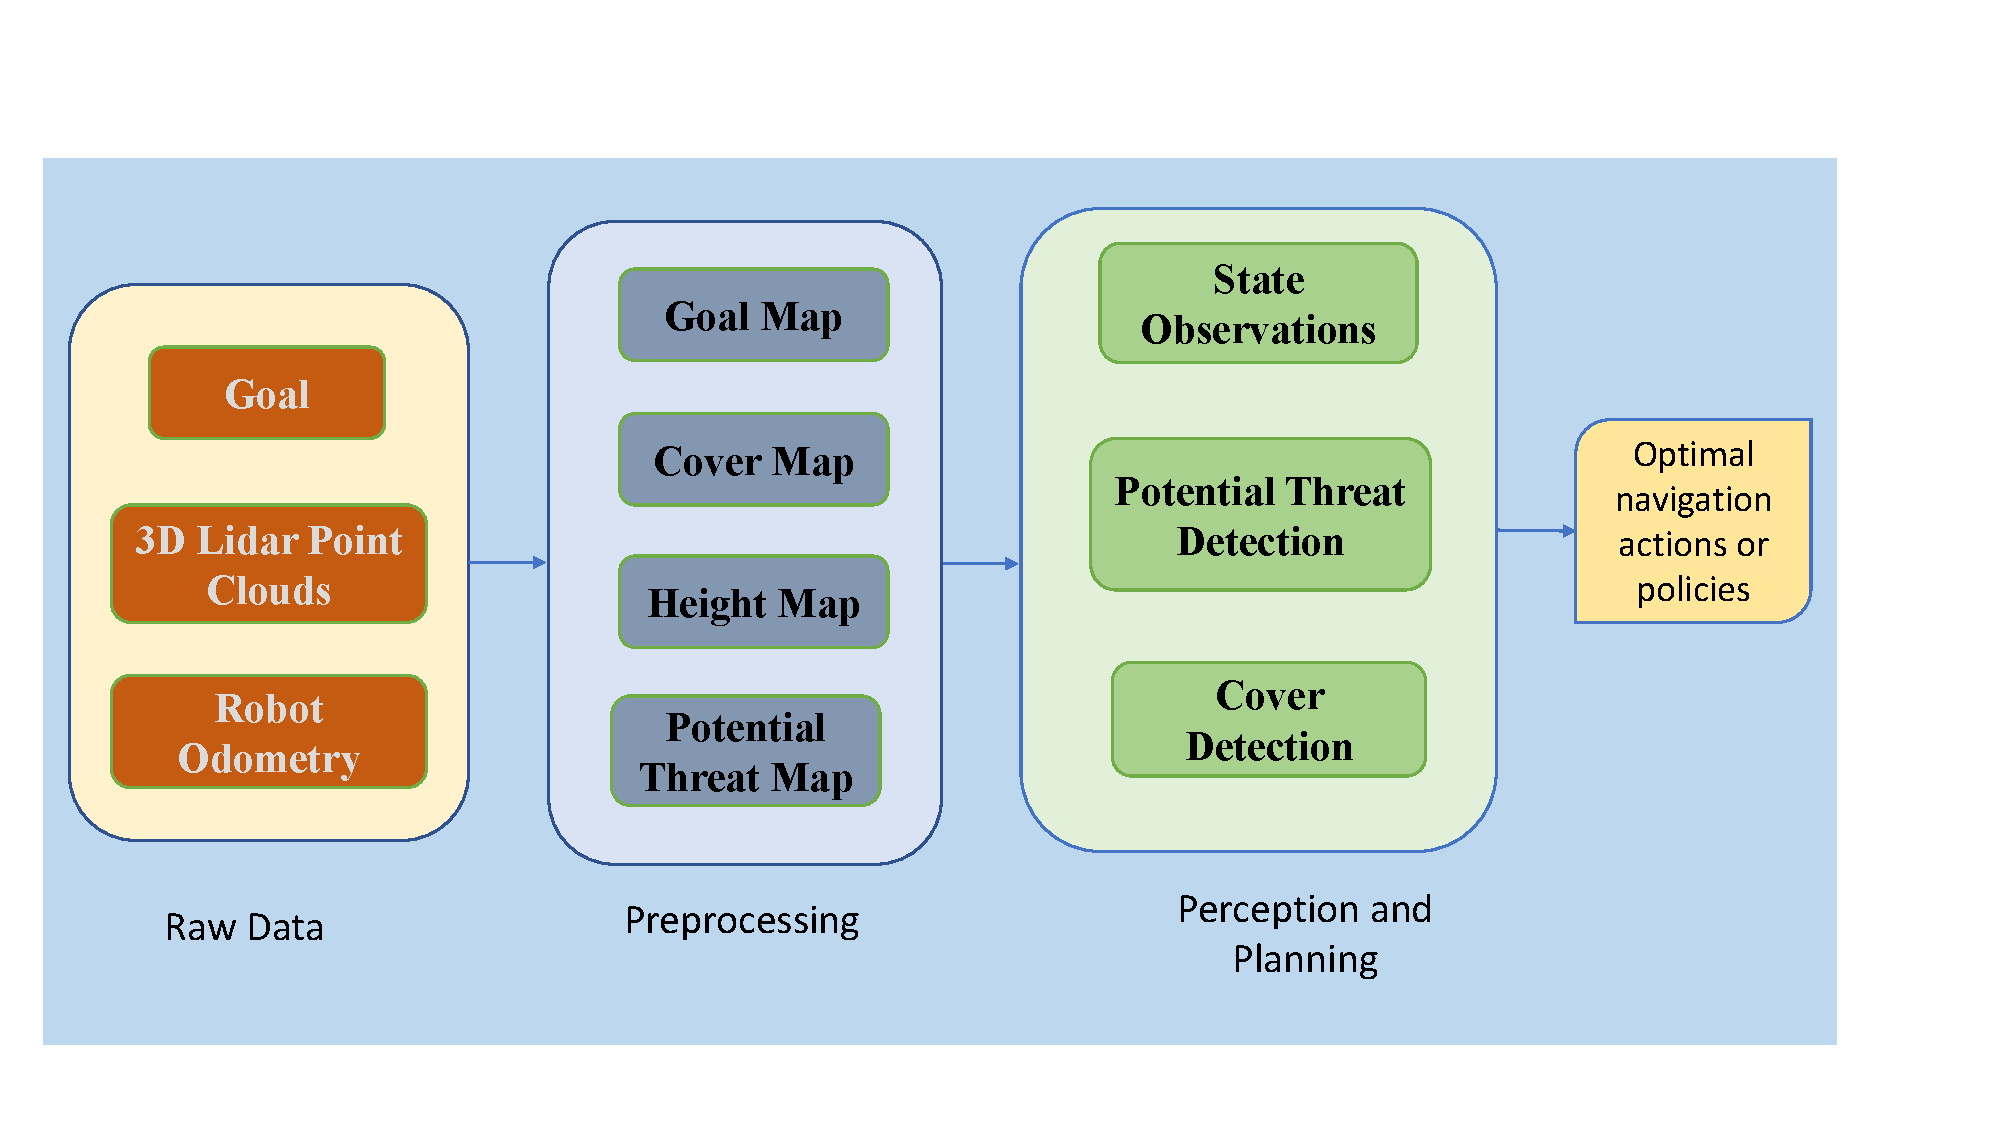
\includegraphics[trim=0cm 0cm 2cm 2cm, clip,width=\linewidth]{sections/images/EnCoMP_Architecture_Updated.pdf}
    \caption{Overview of \textit{EnCoMP} System Architecture.} 
    \label{fig:architecture}
\end{figure}
\subsection{Finding Cover in the Environment}
To identify cover objects in the environment, we process the LiDAR point cloud $\mathcal{P} = \{\mathbf{p}_i \in \mathbb{R}^3 \mid i = 1, \dots, N\}$, where each point $\mathbf{p}_i$ is represented by its 3D coordinates $(x_i, y_i, z_i)$. We apply the following steps:

\textbf{Point Cloud Segmentation:} We use the Euclidean cluster extraction algorithm to segment the point cloud into distinct objects. The algorithm groups nearby points based on their Euclidean distance, forming clusters $\mathcal{C}_j \subset \mathcal{P}$, where $j = 1, \dots, M$ and $M$ is the number of clusters.

\textbf{Cover Object Identification:} For each cluster $\mathcal{C}_j$, we calculate its height $h_j$, density $d_j$, and volume $v_j$ as follows:
\begin{align}
h_j &= \max_{\mathbf{p}_i \in \mathcal{C}_j} z_i - \min_{\mathbf{p}_i \in \mathcal{C}_j} z_i, \\
d_j &= \frac{|\mathcal{C}_j|}{v_j}, \\
v_j &= (x_{j,\max} - x_{j,\min}) \times (y_{j,\max} - y_{j,\min}) \times h_j,
\end{align}
where $|\mathcal{C}_j|$ is the number of points in cluster $\mathcal{C}_j$, and $x_{j,\min}, x_{j,\max}, y_{j,\min}, y_{j,\max}$ are the minimum and maximum coordinates of the cluster in the $x$ and $y$ dimensions, respectively. A cluster $\mathcal{C}_j$ is considered a cover object if it satisfies the following criteria:
\begin{align}
h_j &\geq h_{\min}, \\
d_j &\geq d_{\min}, \\
v_j &\geq v_{\min},
\end{align}
where $h_{\min}, d_{\min}, v_{\min}$ are predefined thresholds for height, density, and volume, respectively where $|\mathcal{C}_j|$ is the number of points in cluster $\mathcal{C}_j$, and $x_{j,\min}, x_{j,\max}, y_{j,\min}, y_{j,\max}$ are the minimum and maximum coordinates of the cluster in the $x$ and $y$ dimensions, respectively.

\subsection{Generating Cover Maps}
The cover map $\mathcal{M}_c$ is a 2D grid representation of the environment, where each cell $(i, j)$ contains the cover density value $c_{i,j} \in [0, 1]$. We generate the cover map using the identified cover objects as follows:

\begin{enumerate}
    \item Initialize the cover map $\mathcal{M}_c$ with dimensions $H \times W$ and cell size $\delta$.
    \item For each cover object $\mathcal{C}_j$, project its points onto the corresponding cells in the cover map. The projection of a point $\mathbf{p}_i = (x_i, y_i, z_i)$ to a cell $(i, j)$ is given by:
    \begin{align}
    i &= \left\lfloor \frac{x_i - x_{\min}}{\delta} \right\rfloor, \\
    j &= \left\lfloor \frac{y_i - y_{\min}}{\delta} \right\rfloor,
    \end{align}
    where $x_{\min}, y_{\min}$ are the minimum coordinates of the environment in the $x$ and $y$ dimensions, respectively.
    \item For each cell $(i, j)$ in the cover map, calculate the cover density $c_{i,j}$ as:
    \begin{equation}
    c_{i,j} = \frac{|\mathcal{P}_{i,j}^c|}{|\mathcal{P}_{i,j}|},
    \end{equation}
    where $\mathcal{P}_{i,j}$ is the set of all LiDAR points projected onto cell $(i, j)$, and $\mathcal{P}_{i,j}^c \subseteq \mathcal{P}_{i,j}$ is the subset of points belonging to cover objects.
\end{enumerate}

% \subsection{Generating Potential Threat Maps}
% The potential threat map $\mathcal{M}_t$ is a 2D grid representation of the environment, where each cell $(i, j)$ contains the potential threat level $t_{i,j} \in [0, 1]$. We generate the potential threat map using the following steps:

% \begin{enumerate}
%     \item Initialize the potential threat map $\mathcal{M}_t$ with the same dimensions and cell size as the cover map.
%     \item Randomly place $K$ potential threats in the environment at locations $\mathbf{t}_k = (x_k, y_k), k = 1, \dots, K$.
%     \item For each cell $(i, j)$ in the potential threat map, calculate the potential threat level $t_{i,j}$ as:
%     \begin{equation}
%     t_{i,j} = \max_{k=1}^{K} \left( \frac{1}{d_{i,j,k}} \right) \cdot \mathbbm{1}[\text{LOS}(\mathbf{p}_{i,j}, \mathbf{t}_k)],
%     \end{equation}
%     where $d_{i,j,k}$ is the Euclidean distance between the center of cell $(i, j)$, denoted as $\mathbf{p}_{i,j}$, and the $k$-th potential threat location $\mathbf{t}_k$. $\mathbbm{1}[\text{LOS}(\mathbf{p}_{i,j}, \mathbf{t}_k)]$ is an indicator function that equals 1 if there is a line of sight between $\mathbf{p}_{i,j}$ and $\mathbf{t}_k$, and 0 otherwise. 
%     % The line of sight is determined using  Bresenham's ray tracing algorithm \cite{wiki_bresenham}.
% \end{enumerate}


% To determine the line-of-sight visibility efficiently, we employ the Discrete Visibility Computation (DVC) algorithm ~\cite{bungiu2014efficient, huynh2024optimizing}. DVC is a state-of-the-art algorithm that computes the visibility of each cell in a 2D grid environment from a given observer position by exploiting the geometric properties of the environment.
% The DVC algorithm works by discretizing the environment into a 2D grid and computing the visibility of each cell using a combination of ray casting and angular sweeping techniques. It efficiently determines the cells that are visible from the observer position by considering the elevation and distance of the cells, as well as the presence of occluding obstacles in the environment.
% DVC achieves a significant speedup compared to traditional line-of-sight computation methods by leveraging the discrete nature of the grid representation and employing efficient data structures, such as binary search trees, to store and query the visibility information.
% By incorporating DVC into our threat map generation process, we can efficiently determine the line-of-sight visibility between each cell and the potential threats in the environment. This enables us to calculate the threat level for each cell more accurately and in real-time, considering both the distance to the threats and the presence of occlusions in the environment.
% The integration of the Discrete Visibility Computation algorithm enhances the efficiency and accuracy of our threat map generation process, allowing the robot to make informed decisions about potential threats and plan paths that minimize the risk of detection.

\subsection{Generating Height Maps}
The height map $\mathcal{M}_h$ is a 2D grid representation of the environment, where each cell $(i, j)$ contains the maximum height value $h_{i,j} \in \mathbb{R}$. We generate the height map using the LiDAR point cloud as follows:

\begin{enumerate}
    \item Initialize the height map $\mathcal{M}_h$ with the same dimensions and cell size as the cover map.
    \item For each LiDAR point $\mathbf{p}_i = (x_i, y_i, z_i)$, project it onto the corresponding cell $(i, j)$ in the height map using the projection equations defined earlier.
    \item For each cell $(i, j)$ in the height map, calculate the maximum height value $h_{i,j}$ as:
    \begin{equation}
    h_{i,j} = \max_{\mathbf{p}_i \in \mathcal{P}_{i,j}} z_i,
    \end{equation}
    where $\mathcal{P}_{i,j}$ is the set of all LiDAR points projected onto cell $(i, j)$.
\end{enumerate}

\subsection{Generating Goal Maps}
The goal map $\mathcal{M}_g$ is a 2D grid representation of the environment, where each cell $(i, j)$ contains a value indicating the relative distance and direction to the goal position. We generate the goal map as follows:
\begin{enumerate}
    \item Initialize the goal map $\mathcal{M}_g$ with the same dimensions and cell size as the cover map and height map.
    \item Set the goal position $(x_g, y_g)$ in the goal map.
    \item For each cell $(i, j)$ in the goal map, calculate the distance $d_{i,j}$ and angle $\theta_{i,j}$ to the goal position:
    \begin{equation}
    d_{i,j} = \sqrt{(x_i - x_g)^2 + (y_j - y_g)^2}
    \end{equation}
    \begin{equation}
    \theta_{i,j} = \text{atan2}(y_j - y_g, x_i - x_g)
    \end{equation}
    \item Normalize the distance values to the range $[0, 1]$ based on the maximum distance in the goal map.
    \item Encode the distance and angle information into the goal map $\mathcal{M}_g$, where each cell contains a tuple $(d_{i,j}, \theta_{i,j})$.
\end{enumerate}
The goal map provides the robot with information about the relative distance and direction to the goal position, guiding its navigation towards the target location.


% \subsection{Adaptive Threat-Aware Visibility Estimation (ATAVE)}
% \label{subsec:atave}

% The Adaptive Threat-Aware Visibility Estimation (ATAVE) algorithm ~\ref{alg:atave} is a pivotal component of the EnCoMP system, designed to optimize navigation strategies by dynamically assessing and mitigating potential threats in real-time.



% \begin{algorithm}
% \caption{Adaptive Threat-Aware Visibility Estimation (ATAVE)}
% \label{alg:atave}
% \SetAlgoLined
% \KwData{Environment $\mathcal{E}$, cells $\mathcal{C}$, robot position $r$, trajectory $\mathcal{T}_{path}$, cover map $\mathcal{M}_c$}
% \KwResult{Threat assessment $\phi(c_i, \mathcal{T}_{path})$ for each $c_i$}

% \textbf{Initialize:} $p_t(c_i)$ for all $c_i$\;
% \textbf{Build Tree:} $\mathcal{T}_{tree}$ from threat probabilities\;

% \ForEach{$c_i \in \mathcal{C}$}{
%     Compute visibility $v(c_i, r)$ using LLA: $v(c_i, r) = \text{LLA}(\mathcal{T}_{tree}, c_i, r)$\;
%     Assess threat $\tau(c_i, r)$: $\tau(c_i, r) = \max_{v_j} v(c_i, v_j) \cdot p_t(v_j)$\;
%     Predict visibility $\rho(c_i, \mathcal{T}_{path})$: $\rho(c_i, \mathcal{T}_{path}) = \max_{r_k} \tau(c_i, r_k) \cdot \gamma^k$\;
%     Evaluate threat $\phi(c_i, \mathcal{T}_{path})$: $\phi(c_i, \mathcal{T}_{path}) = \rho(c_i, \mathcal{T}_{path}) \cdot (1 - \mathcal{M}_c(c_i))$\;
% }

% \While{robot is navigating}{
%     Update $p_t(c_i)$ with new data $o_t$: $p_t(c_i) = \frac{p_{t-1}(c_i) \cdot p(o_t | c_i)}{\sum_{c_j \in \mathcal{C}} p_{t-1}(c_j) \cdot p(o_t | c_j)}$\;
%     Recompute $\phi(c_i, \mathcal{T}_{path})$ for all $c_i$\;
%     Select next action based on $\phi(c_i, \mathcal{T}_{path})$\;
% }
% \end{algorithm}

% At the core of ATAVE is a probabilistic threat model $p_t(c_i)$ maintained for each cell $c_i$ in the discretized environment $\mathcal{C}$. This model represents the likelihood of a threat being present in each cell at time $t$. The threat probabilities are initially estimated based on prior knowledge and are continuously updated using the robot's observations and sensor data through a Bayesian update process:
% \begin{equation}
% p_t(c_i) = \frac{p_{t-1}(c_i) \cdot p(o_t | c_i)}{\sum_{j=1}^{N} p_{t-1}(c_j) \cdot p(o_t | c_j)}
% \end{equation}
% where $p_{t-1}(c_i)$ is the prior probability of a threat in cell $c_i$ at time $t-1$, $p(o_t | c_i)$ is the likelihood of observing data $o_t$ given a threat in cell $c_i$, and the denominator ensures normalization.


% To provide a comprehensive assessment of the risk associated with each cell, ATAVE employs a multi-perspective threat estimation approach. It considers the robot's visibility from multiple vantage points, denoted as $\mathcal{V} = {v_1, v_2, \ldots, v_M}$, representing potential threat perspectives. The multi-perspective threat assessment is computed as:
% \begin{equation}
% \tau(c_i, r) = \max_{v_j \in \mathcal{V}} v(c_i, v_j) \cdot p_t(v_j)
% \end{equation}
% where $\tau(c_i, r)$ represents the multi-perspective threat assessment of cell $c_i$ from the robot's position $r$, $v(c_i, v_j)$ is the visibility of cell $c_i$ from vantage point $v_j$, and $p_t(v_j)$ is the probability of a threat being present at vantage point $v_j$.
% To enable real-time threat assessment, ATAVE utilizes efficient visibility computation techniques, such as the Late Line-of-Sight Check and Prioritized Tree Structures (LLA) ~\cite{Zhang2019LateLC}. These techniques significantly reduce the computational overhead while maintaining high accuracy in determining the robot's visibility from different threat perspectives.
% Based on the dynamic threat assessment, ATAVE continuously adapts the robot's navigation strategy to minimize exposure to high-risk areas. It integrates with the cover utilization and path planning components of EnCoMP to generate safer and more efficient trajectories that prioritize covert operation. The cover-aware threat assessment for a cell $c_i$ along the robot's planned trajectory $\mathcal{T}$ is computed as:
% \begin{equation}
% \phi(c_i, \mathcal{T}) = \rho(c_i, \mathcal{T}) \cdot (1 - \mathcal{M}_c(c_i))
% \end{equation}
% where $\phi(c_i, \mathcal{T})$ represents the cover-aware threat assessment of cell $c_i$ along trajectory $\mathcal{T}$, $\rho(c_i, \mathcal{T})$ is the temporal visibility prediction of cell $c_i$ along trajectory $\mathcal{T}$, and $\mathcal{M}_c(c_i)$ is the cover density of cell $c_i$.
% By integrating ATAVE's dynamic threat assessment and adaptive navigation capabilities, EnCoMP enables autonomous robots to effectively operate in complex and dynamic environments. The probabilistic threat modeling, multi-perspective threat estimation, efficient visibility computation, and cover-aware navigation planning allow the robot to maintain high situational awareness, adapt to evolving threats, and prioritize covert operation while efficiently reaching its goal. As shown in Figure~\ref{fig:llastar_visibility}, the LLA* algorithm efficiently computes the visibility of cells from the threat's perspective, enabling the robot to assess the risk of detection and make informed decisions during navigation.


\subsection{Adaptive Threat-Aware Visibility Estimation (ATAVE)}
\label{subsec:atave}
The Adaptive Threat-Aware Visibility Estimation (ATAVE) algorithm (see Algorithm~\ref{alg:atave}) is a pivotal component of the \textit{EnCoMP} system, designed to optimize navigation strategies by dynamically assessing and mitigating potential threats in real-time.

\begin{algorithm}
\caption{Adaptive Threat-Aware Visibility Estimation (ATAVE)}
\label{alg:atave}
\SetAlgoLined
\KwData{Environment $\mathcal{E}$, cells $\mathcal{C}$, robot position $r$, trajectory $\mathcal{T}_{\text{path}}$, cover map $\mathcal{M}_c$, goal map $\mathcal{M}_g$}
\KwResult{Threat assessment $\phi(c_i, \mathcal{T}_{\text{path}})$ for each $c_i$}
\textbf{Initialize:} $p_t(c_i)$ for all $c_i$\;
\textbf{Build Tree:} $\mathcal{T}_{\text{tree}}$ from threat probabilities\;
\ForEach{$c_i \in \mathcal{C}$}{
    Compute visibility $v(c_i, r)$ using LLA: $v(c_i, r) = \text{LLA}(\mathcal{T}_{\text{tree}}, c_i, r)$\;
    Assess threat $\tau(c_i, r)$: $\tau(c_i, r) = \max_{v_j} v(c_i, v_j) \cdot p_t(v_j)$\;
    Predict visibility $\rho(c_i, \mathcal{T}_{\text{path}})$: $\rho(c_i, \mathcal{T}_{\text{path}}) = \max_{r_k} \tau(c_i, r_k) \cdot \gamma^k$\;
    Evaluate threat $\phi(c_i, \mathcal{T}_{\text{path}})$: $\phi(c_i, \mathcal{T}_{\text{path}}) = \rho(c_i, \mathcal{T}_{\text{path}}) \cdot (1 - \mathcal{M}_c(c_i)) \cdot \mathcal{M}_g(c_i)$\;
}
\While{robot is navigating}{
    Update $p_t(c_i)$ with new data $o_t$: $p_t(c_i) = \frac{p_{t-1}(c_i) \cdot p(o_t | c_i)}{\sum_{c_j \in \mathcal{C}} p_{t-1}(c_j) \cdot p(o_t | c_j)}$\;
    Recompute $\phi(c_i, \mathcal{T}_{\text{path}})$ for all $c_i$\;
    Select next action based on $\phi(c_i, \mathcal{T}_{\text{path}})$\;
}
\end{algorithm}

At the core of ATAVE is a probabilistic threat model $p_t(c_i)$ maintained for each cell $c_i$ in the discretized environment $\mathcal{C}$. This model represents the likelihood of a threat being present in each cell at time $t$. The threat probabilities are initially estimated based on prior knowledge and are continuously updated using the robot's observations and sensor data through a Bayesian update process:
\begin{equation}
p_t(c_i) = \frac{p_{t-1}(c_i) \cdot p(o_t | c_i)}{\sum_{j=1}^{N} p_{t-1}(c_j) \cdot p(o_t | c_j)}
\end{equation}

where $p_{t-1}(c_i)$ is the prior probability of a threat in cell $c_i$ at time $t-1$, $p(o_t | c_i)$ is the likelihood of observing data $o_t$ given a threat in cell $c_i$, and the denominator ensures normalization.
To provide a comprehensive assessment of the risk associated with each cell, ATAVE employs a multi-perspective threat estimation approach. It considers the robot's visibility from multiple vantage points, denoted as $\mathcal{V} = \{v_1, v_2, \ldots, v_M\}$, representing potential threat perspectives. The multi-perspective threat assessment is computed as:
\begin{equation}
\tau(c_i, r) = \max_{v_j \in \mathcal{V}} v(c_i, v_j) \cdot p_t(v_j)
\end{equation}

where $\tau(c_i, r)$ represents the multi-perspective threat assessment of cell $c_i$ from the robot's position $r$, $v(c_i, v_j)$ is the visibility of cell $c_i$ from vantage point $v_j$, and $p_t(v_j)$ is the probability of a threat being present at vantage point $v_j$.
To enable real-time threat assessment, ATAVE utilizes efficient visibility computation techniques, such as the Late Line-of-Sight Check and Prioritized Tree Structures (LLA) \cite{Zhang2019LateLC}. These techniques significantly reduce the computational overhead while maintaining high accuracy in determining the robot's visibility from different threat perspectives. As shown in Figure~\ref{fig:llastar_visibility}, the LLA* algorithm efficiently computes the visibility of cells from the threat's perspective, enabling the robot to assess the risk of detection and make informed decisions during navigation.


The goal map $\mathcal{M}_g$ is also utilized in the ATAVE algorithm to guide the robot's navigation while considering the threat exposure. The cover-aware threat assessment for a cell $c_i$ along the robot's planned trajectory $\mathcal{T}$ is computed as:
\begin{equation}
\phi(c_i, \mathcal{T}) = \rho(c_i, \mathcal{T}) \cdot (1 - \mathcal{M}_c(c_i)) \cdot \mathcal{M}_g(c_i)
\end{equation}

where $\phi(c_i, \mathcal{T})$ represents the cover-aware threat assessment of cell $c_i$ along trajectory $\mathcal{T}$, $\rho(c_i, \mathcal{T})$ is the temporal visibility prediction of cell $c_i$ along trajectory $\mathcal{T}$, $\mathcal{M}_c(c_i)$ is the cover density of cell $c_i$, and $\mathcal{M}_g(c_i)$ is the goal map value of cell $c_i$, indicating its proximity and direction to the goal.
By incorporating the goal map into the cover-aware threat assessment, ATAVE prioritizes navigation decisions that balance the objectives of minimizing threat exposure, maximizing cover utilization, and progressing towards the goal. 

% This integration allows the robot to make informed decisions that adapt to the complex environment while maintaining a goal-oriented behavior.
% Based on the dynamic threat assessment, ATAVE continuously adapts the robot's navigation strategy to minimize exposure to high-risk areas. It integrates with the cover utilization and path planning components of \textit{EnCoMP} to generate safer and more efficient trajectories that prioritize covert operations.


\textbf{Proposition V.1.} \textit{The ATAVE algorithm modifies the threat exposure function \(\varphi(c_i, T_{path})\) such that traversability costs in high-threat regions are always higher than those in low-threat regions.} 

\textbf{Proof.} Consider the cover-aware threat assessment function \(\varphi(c_i, T_{path})\) used in the ATAVE algorithm: \(\varphi(c_i, T_{path}) = \rho(c_i, T_{path}) \cdot (1 - M_c(c_i)) \cdot M_g(c_i)\) where \(\rho(c_i, T_{path})\) is the temporal visibility prediction of cell \(c_i\) along the trajectory \(T_{path}\), \(M_c(c_i)\) is the cover density of cell \(c_i\), and \(M_g(c_i)\) is the goal map value of cell \(c_i\). The maximum cost for a region with low cover density (high visibility and threat probability) can be expressed as: \(\varphi_{\max} = \rho_{\max} \cdot (1 - M_{c_{\min}}) \cdot M_{g_{\max}}\) where \(\rho_{\max}\) is the maximum visibility prediction, \(M_{c_{\min}}\) is the minimum cover density (which is 0 for no cover), and \(M_{g_{\max}}\) is the maximum goal map value. The minimum cost for a region with high cover density (low visibility and threat probability) can be expressed as: \(\varphi_{\min} = \rho_{\min} \cdot (1 - M_{c_{\max}}) \cdot M_{g_{\min}}\) where \(M_{c_{\max}}\) is the maximum cover density (which is 1 for full cover), \(\rho_{\min}\) is the minimum visibility prediction, and \(M_{g_{\min}}\) is the minimum goal map value. Given \(M_{c_{\max}} = 1\) and assuming \(\rho_{\min}\) and \(M_{g_{\min}}\) are non-zero, this simplifies to: \(\varphi_{\min} = 0\). Since \(\rho_{\max} \cdot (1 - M_{c_{\min}}) \cdot M_{g_{\max}} > 0\), it follows that: \(\varphi_{\max} > \varphi_{\min}\). 

Therefore, the ATAVE algorithm assigns higher costs to regions with higher visibility and threat probability. Consequently, the agent, following the path of least cost, will prefer navigating through regions with higher cover density and lower visibility and threat probability. Thus, regions with lower threat exposure will always be preferred for navigation. \(\blacksquare\)


\begin{figure}[!htb]
    \centering
    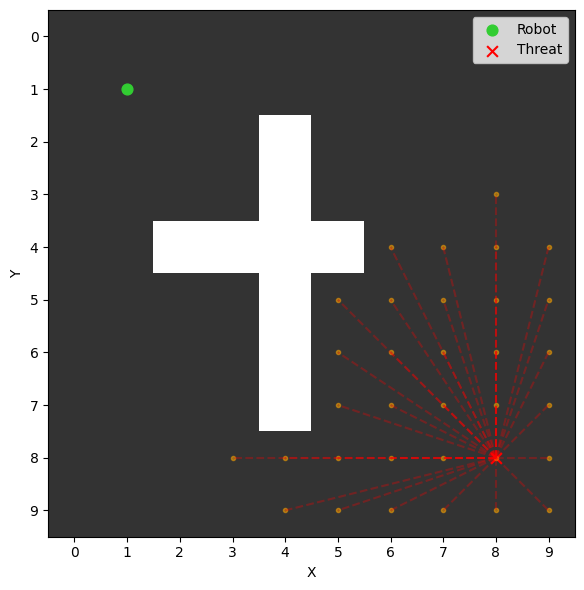
\includegraphics[width=\linewidth]{sections/images/visibility_calculation.png}
    \caption{Visualization of the LLA* Visibility Calculation in the \textit{EnCoMP} framework. The plot shows the grid environment with obstacles (gray cells), the robot's position (green circle), the threat's position (red cross), and the visible cells (orange dots) determined by the Late Line-of-Sight Check and Prioritized Trees (LLA*) algorithm. The red dashed lines represent the line-of-sight from the threat to the visible cells within its visibility range. }
   \label{fig:llastar_visibility}
\end{figure}


\subsection{Reward Functions}

We design the following reward functions to capture the objectives of the covert navigation problem:

\textbf{Cover Utilization Reward : }The cover utilization reward encourages the robot to navigate through areas with high cover density, as indicated by the cover map $\mathcal{C}$. It is defined as:

\begin{equation}
R_{\text{cover}}(s, a) = \lambda_c \sum_{i=1}^{M} \sum_{j=1}^{N} \mathcal{C}_{ij} \cdot \mathbbm{1}\left[(x_i, y_j) \in \xi(s, a)\right]
\end{equation}

where $\lambda_c$ is a positive weighting factor, $\mathcal{C}_{ij}$ is the cover density value at cell $(i, j)$ in the cover map, $\mathbbm{1}[\cdot]$ is the indicator function, and $\xi(s, a)$ is the set of cells traversed by the robot when taking action $a$ in state $s$.

\textbf{Threat Exposure Penalty : } The threat exposure penalty discourages the robot from being exposed to potential threats, as indicated by the potential threat map $\mathcal{T}$. It is defined as:

\begin{equation}
R_{threat}(s) = -\lambda_t \sum_{i=1}^{M} \sum_{j=1}^{N} \mathcal{T}_{ij} \cdot \mathbbm{1}[(x_i, y_j) \in \xi(s)]
\end{equation}

where $\lambda_t$ is a weighting factor, $\mathcal{T}_{ij}$ is the threat level at cell $(i, j)$ in the potential threat map, and $\xi(s)$ is the set of cells occupied by the robot in state $s$.

\textbf{Goal Reaching Reward : }The goal reaching reward encourages the robot to make progress towards the goal position. It is defined as:

\begin{equation}
R_{goal}(s, a) = \lambda_g (d(s, g) - d(s', g))
\end{equation}

where $\lambda_g$ is a positive weighting factor, $d(s, g)$ is the distance between the robot's position in state $s$ and the goal position $g$, and $s'$ is the state reached after taking action $a$ in state $s$.

\textbf{Collision Penalty : }The collision penalty discourages the robot from colliding with obstacles or navigating through untraversable regions, as indicated by the height map $\mathcal{H}$. It is defined as:

\begin{equation}
R_{\text{collision}}(s, a) = 
\begin{cases}
-\lambda_o, & \text{if } \exists (x_i, y_j) \in \xi(s, a), \mathcal{H}_{ij} > h_{\max}, \\
0, & \text{otherwise.}
\end{cases}
\end{equation}



where $\lambda_o$ represents the weight assigned to the collision penalty, $\mathcal{H}_{ij}$ is the height value at cell $(i, j)$ in the height map, and $h_{max}$ is the maximum traversable height threshold.

\subsection{CQL Policy Learning with Multi-Map Inputs}

We employ Conservative Q-Learning (CQL) ~\cite{kumar2020conservative} to learn the covert navigation policy from the diverse dataset $\mathcal{D}$ collected from real-world environments. CQL learns a conservative estimate of the Q-function by incorporating a regularization term in the training objective, which encourages the learned Q-function to assign lower values to out-of-distribution actions while still accurately fitting the Q-values for actions observed in the dataset. The CQL objective is defined as:

\begin{equation}
\begin{split}
\mathcal{L}(\theta) = \mathbb{E}_{(\mathbf{s}, \mathbf{a}, r, \mathbf{s}') \sim \mathcal{D}} \Big[ &(Q_\theta(\mathbf{s}, \mathbf{a}) - \\
&(r + \gamma \mathbb{E}_{\mathbf{a}' \sim \pi_\theta(\cdot \mid \mathbf{s}')}[Q_\theta(\mathbf{s}', \mathbf{a}')]))^2 \Big] \\
&+ \alpha \mathcal{R}(\theta)
\end{split}
\end{equation}


where $Q_\theta$ is the Q-function parameterized by $\theta$, $\pi_\theta$ is the policy, $\alpha$ is a hyperparameter controlling the strength of the regularization term $\mathcal{R}(\theta)$, and $\mathcal{D}$ is the dataset of transitions.

The regularization term $\mathcal{R}(\theta)$ is defined as:

\begin{equation}
\begin{split}
\mathcal{R}(\theta) = \mathbb{E}_{\mathbf{s} \sim \mathcal{D}} \bigg[ &\log \sum_{\mathbf{a}} \exp(Q_\theta(\mathbf{s}, \mathbf{a})) \\
&- \mathbb{E}_{\mathbf{a} \sim \pi_\beta(\cdot \mid \mathbf{s})}[Q_\theta(\mathbf{s}, \mathbf{a})] \bigg]
\end{split}
\end{equation}


where $\pi_\beta$ is the behavior policy used to collect the dataset $\mathcal{D}$. To learn the covert navigation policy, we use the high-fidelity cover map $\mathcal{C}$, potential threat map $\mathcal{T}$, height map $\mathcal{H}$, and goal map $\mathcal{M}_g$ as input to the Q-function and policy networks. The state input to the networks is defined as:
\begin{equation}
s = [\mathcal{C}, \mathcal{T}, \mathcal{H}, \mathcal{M}_g, p_r, p_g]
\end{equation}
where $p_r$ and $p_g$ are the robot's position and goal position, respectively.

During training, the CQL algorithm samples batches of transitions $(\mathbf{s}, \mathbf{a}, r, \mathbf{s}')$ from the dataset $\mathcal{D}$ and updates the Q-function and policy networks using the CQL objective. The Q-function network learns to estimate the expected cumulative reward for each state-action pair, while the policy network learns to select actions that maximize the Q-values. By incorporating the multi-map inputs and utilizing the conservative Q-learning objective, the learned policy effectively navigates the robot towards the goal while maximizing cover utilization, minimizing threat exposure, and avoiding collisions. The CQL algorithm ensures that the learned policy is robust and generalizes well to novel environments by penalizing overestimation of Q-values for out-of-distribution actions.

During deployment, the learned policy takes the current state $\mathbf{s}$, which includes the multi-map inputs, and outputs the optimal action $\mathbf{a}^*$ to navigate the robot covertly and efficiently. The robot executes the selected action and observes the next state $\mathbf{s}'$ and reward $r$. This process is repeated until the robot reaches the goal or a maximum number of steps is reached,  which serves as the failure condition. By leveraging the map inputs and the CQL algorithm, our approach learns a robust and efficient policy for covert navigation in complex environments, enabling the robot to make informed decisions based on the comprehensive understanding of the environment provided by the cover map, potential threat map, and height map.
% \begin{equation}
% \mathbf{a}^* = \pi_\theta(\mathbf{s})
% \end{equation}


\subsection{Threat-Aware Cover-Based Planning}

% In our framework, the Adaptive Threat-Aware Visibility Estimation (ATAVE) enhances the adaptive covert navigation system by dynamically adjusting action selection based on threat awareness and environmental context. We employ a threat-aware planning algorithm where each action \(a\) from the set \(A\) is evaluated using \(Q_{\text{min}}(s, a; \theta)\). This evaluation incorporates the current state \(s\) and the parameters \(\theta\) of our model, assessing the viability of actions within the defined action space \(V_s = \{(v_x, v_y, \omega_z)\}\).

% ATAVE specifically tailors the velocity constraints \(v = (v_x, v_y)\) and angular velocity \(\omega_z\) based on the robot's ability to minimize detectability while maximizing navigational efficiency. The action space is dynamically adjusted, taking into account both the robot's physical constraints and the detected environmental threats, to provide a balance between agility and stealth. Crucially, ATAVE integrates real-time visibility estimations to proactively modify the robot's trajectory. This adjustment is informed by calculated threat levels from potential detection points, allowing the robot to effectively minimize its visibility to threats. As it navigates through varied terrains, the robot utilizes environmental features such as tree density and urban structures to remain undetected, strategically adapting its path to make use of available cover and avoid exposed areas.

% The decision-making model utilizes the restricted velocity space \(V_s\), which adapts based on real-time environmental data and threat assessments:
% \[
% V_s = 
% \begin{cases} 
% (v_x, v_y, 0), & \text{if minimal threat is detected} \\
% (v_x, 0, \omega_z), & \text{otherwise}
% \end{cases}
% \]

% This structured adaptation ensures that each selected action \(a^*\) strategically minimizes threat exposure while promoting effective progress towards the navigation goal:
% \[
% a^* = \arg\min_{a \in A} Q_{\text{min}}(s, a).
% \]

% By integrating the ATAVE method, our navigation system not only leverages the robotic platform's capabilities but also actively responds to changing environmental dynamics. This approach ensures that the navigation system is both effective and secure, capable of adapting in real-time to complex and evolving landscapes.

% To dynamically generate feasible actions , we develop an enhanced covert maneuver planner that strategy adjusts the robot's velocity and trajectory based on continuously updated threat assessments, balancing stealth with navigational efficiency in complex environments.

% \subsection{Threat-Aware Cover-Based Planning}
% To dynamically generate feasible actions, we develop an enhanced covert maneuver planner that strategically adjusts the robot's velocity and trajectory based on continuously updated threat assessments, balancing stealth with navigational efficiency in complex environments. Our ATAVE-driven algorithm modifies the robot’s velocity set \(V_s\) in real-time to align with varying threat levels:
% \[
% V_s = 
% \begin{cases} 
% (v_x, v_y, 0), & \text{if minimal threat is detected} \\
% (v_x, 0, \omega_z), & \text{otherwise}
% \end{cases}
% \]
% This velocity configuration allows the robot to navigate efficiently in low-risk situations by moving freely in the horizontal plane (\(v_x\) and \(v_y\)) without rotational movements (\(\omega_z = 0\)). Such freedom is crucial for rapid traversal in environments where detection risks are minimal. Conversely, in higher threat scenarios, the robot's movement is restricted to the \(z\)-axis rotations and forward movement along the \(x\)-axis, with lateral movements (\(v_y\)) eliminated to minimize the robot’s detectability. This selective restriction aids the robot in using the environment strategically—such as navigating closer to natural or man-made covers—which significantly enhances concealment.

% The adaptability of our velocity control strategy, \(V_s\), exemplifies proactive threat management, enabling the robot to make intelligent navigation decisions that reduce its visibility to potential threats while maximizing cover effectiveness. 


% To effectively handle covert navigation in complex environments, we design a dynamic action selection strategy that utilizes an enhanced covert maneuver planner. For our robot, an action \(a\) from the set of all possible actions \(A\) is evaluated using \(Q_{\min}(s, a; \theta)\), where \(s\) is the current state and \(\theta\) represents the parameters of our model. The action space \(V_s\) is defined based on the robot's operational capabilities and the environmental context:
% \[
% V_s = 
% \begin{cases} 
% (v_x, v_y, 0), & \text{if minimal threat is detected} \\
% (v_x, 0, \omega_z), & \text{otherwise}
% \end{cases}
% \]
% This configuration of \(V_s\) allows the robot to adjust its velocity dynamically:
% \begin{itemize}
%     \item When minimal threats are detected, the robot can move freely in both the \(x\) and \(y\) directions on the horizontal plane, optimizing speed and path efficiency without rotational movements (\(\omega_z = 0\)).
%     \item In higher threat scenarios, the robot's movement is constrained to the \(z\)-axis rotations and direct movement along the \(x\)-axis, with lateral movements (\(v_y\)) eliminated to minimize the robot's detectability.
% \end{itemize}

% These values are restricted within their maximum limits to ensure safe and efficient navigation. Specifically, our approach dynamically adjusts the linear and angular velocities based on the terrain and obstacle density, crucial for maintaining stealth and avoiding detection. To optimize the navigation strategy, the robot evaluates potential paths by predicting the outcomes of different actions within its dynamically restricted velocity space \(V_s\). This space is adjusted in real-time based on detected environmental features such as cover availability and potential threat locations. For example, in areas with dense cover, the robot may reduce speed to minimize noise and avoid disturbing the environment, which could lead to detection.

% Moreover, the system prioritizes paths that utilize natural landscape features to enhance covertness, adapting its movement patterns to the context of each specific mission scenario. The decision-making process involves selecting the action \(a^*\) that minimizes exposure to threats while maximizing progress towards the goal, calculated as:
% \[
% a^* = \arg\min_{a \in A} Q_{\min}(s, a).
% \]
% In essence, our adaptive covert navigation framework not only considers the physical capabilities of the robot but also integrates environmental context to make real-time strategic decisions, enhancing the robot's ability to navigate covertly and efficiently across varying terrains.




% To effectively handle covert navigation in complex environments, we design a dynamic action selection strategy that utilizes an enhanced covert maneuver planner. For our robot, an action \(a\) from the set of all possible actions \(A\) is evaluated using \(Q_{\min}(s, a; \theta)\), where \(s\) is the current state and \(\theta\) represents the parameters of our model. The action space \(V_s\) is defined based on the robot's operational capabilities and the environmental context:
% \[
% V_s = (v_x, \omega_z)
% \]
% where \(v_x \in [0, 2.0]\) m/s and \(\omega_z \in [-1.5, 1.5]\) rad/s, reflecting the robot's maximum linear and angular velocities.

% Our approach dynamically adjusts the linear and angular velocities based on the terrain and obstacle density, which is crucial for maintaining stealth and avoiding detection. To optimize the navigation strategy, the robot evaluates potential paths by predicting the outcomes of different actions within its dynamically restricted velocity space \(V_s\). This space is adjusted in real-time based on detected environmental features such as cover availability and potential threat locations. For example, in areas with dense cover, the robot may reduce speed to minimize noise and avoid disturbing the environment, which could lead to detection. Moreover, the system prioritizes paths that utilize natural landscape features to enhance covertness, adapting its movement patterns to the context of each specific mission scenario. The decision-making process involves selecting the action \(a^*\) that minimizes exposure to threats while maximizing progress towards the goal, calculated as:
% \[
% a^* = \arg \min_{a \in A} Q_{\min}(s, a).
% \]
% In essence, our adaptive covert navigation framework not only considers the physical capabilities of the robot but also integrates environmental context to make real-time strategic decisions, enhancing the robot's ability to navigate covertly and efficiently across varying terrains.



To effectively handle covert navigation in complex environments, we design a dynamic action selection strategy that utilizes an enhanced covert maneuver planner. For our robot, an action \(a\) from the set of all possible actions \(A\) is evaluated using \(Q_{\min}(s, a; \theta)\), where \(s\) is the current state and \(\theta\) represents the parameters of our model. The action space \(V_s\) is defined based on the robot's operational capabilities and the environmental context:
\[
V_s =
\begin{cases}
(v_x, \omega_z), & \text{if minimal threat is detected} \\
(v_x', \omega_z'), & \text{otherwise}
\end{cases}
\]
where \(v_x, v_x' \in [0, 2.0]\) m/s and \(\omega_z, \omega_z' \in [-1.5, 1.5]\) rad/s, reflecting the robot's maximum linear and angular velocities.

When minimal threats are detected, the robot can move at its normal speed and angular velocity range. However, in higher threat scenarios, the linear and angular velocities are reduced to \(v_x'\) and \(\omega_z'\), respectively, to minimize the robot's detectability and noise. The dynamic adjustment of velocities is based on the detected threat levels and the surrounding environment. In areas with higher threat levels or dense obstacles, the robot reduces its speed and angular velocity to maintain stealth and avoid detection. The  values of \(v_x'\) and \(\omega_z'\) are determined by functions that take into account the threat level and obstacle density:
\[
v_x' = f_v(\text{threat\_level}, \text{obstacle\_density})
\]
\[
\omega_z' = f_{\omega}(\text{threat\_level}, \text{obstacle\_density})
\]
where \(f_v\) and \(f_{\omega}\) are functions that map the \(\text{threat\_level} \in [0, 1]\)  and \(\text{obstacle\_density} \in [0, 1]\) to appropriate linear and angular velocity values, respectively. These functions are designed to ensure that the robot moves slowly and cautiously in high-threat and dense environments while still making progress towards the goal. Moreover, the system prioritizes paths that utilize natural landscape features to enhance covertness, adapting its movement patterns to the context of each specific mission scenario. The decision-making process involves selecting the action \(a^*\) that minimizes exposure to threats while maximizing progress towards the goal, calculated as:
\[
a^* = \arg\min_{a \in A} Q_{\min}(s, a).
\]
% In essence, our adaptive covert navigation framework not only considers the physical capabilities of the robot but also integrates environmental context and threat levels to make real-time strategic decisions, enhancing the robot's ability to navigate covertly and efficiently across varying terrains.



% The dynamic adjustment of velocities is based on the detected threat levels and the surrounding environment. The specific values of \(v_x'\) and \(\omega_z'\) are determined by the following piecewise linear functions:
% \[
% v_x' =
% \begin{cases}
% 2.0, & \text{if } \text{threat\_level} \leq 0.3 \text{ and } \text{obstacle\_density} \leq 0.2 \\
% 1.5, & \text{if } 0.3 < \text{threat\_level} \leq 0.6 \text{ or } 0.2 < \text{obstacle\_density} \leq 0.4 \\
% 1.0, & \text{if } 0.6 < \text{threat\_level} \leq 0.8 \text{ or } 0.4 < \text{obstacle\_density} \leq 0.6 \\
% 0.5, & \text{otherwise}
% \end{cases}
% \]
% \[
% \omega_z' =
% \begin{cases}
% 1.5, & \text{if } \text{threat\_level} \leq 0.3 \text{ and } \text{obstacle\_density} \leq 0.2 \\
% 1.0, & \text{if } 0.3 < \text{threat\_level} \leq 0.6 \text{ or } 0.2 < \text{obstacle\_density} \leq 0.4 \\
% 0.5, & \text{if } 0.6 < \text{threat\_level} \leq 0.8 \text{ or } 0.4 < \text{obstacle\_density} \leq 0.6 \\
% 0.25, & \text{otherwise}
% \end{cases}
% \]
% where \(\text{threat\_level} \in [0, 1]\) represents the normalized threat level, and \(\text{obstacle\_density} \in [0, 1]\) represents the normalized obstacle density. These functions ensure that the robot moves slowly and cautiously in high-threat and dense environments while still making progress towards the goal.